\documentclass[ 12pt ]{article}
\usepackage{amsmath, amsthm, amssymb, csquotes, enumitem, graphicx, listings, mathrsfs, tikz, pgfplots}
\usepackage[margin=0.5in]{geometry}
\usepgfplotslibrary{fillbetween}
\usetikzlibrary{patterns}
\pgfplotsset{compat=1.12}
\graphicspath{ ./ }


\begin{document}

\noindent Landon Fox \\
\noindent Math 487 \\
\noindent February 5, 2021 \\
\noindent \textbf{Collaborated with Logan Leavitt}

\begin{center}
	\Large Homework 1
\end{center}

\begin{enumerate}
	% problem 1
	\item[\textbf{1.}] Formulate and graphically solve the \textit{The Three Princes of Serendip}.

		\begin{proof}[Solution]
			We are provided that following information:
			\begin{itemize}
				\item No more than 300lb can be carried.
				\item No more than 15$\mathrm{ft}^3$ can be transported.
				\item A coconut has
				\begin{itemize}
					\item a worth of 60 rupees,
					\item a weight of 5lb,
					\item a volume of $\frac{1}{8}\mathrm{ft}^3$.
				\end{itemize}
				\item A lion skin has
				\begin{itemize}
					\item a worth of 300 rupees,
					\item a weight of 15lb,
					\item a volume of 1$\mathrm{ft}^3$.
				\end{itemize}
				\item Optimize profit.
			\end{itemize}
			Let $c, \ell \in \mathbb{R}$ denote the number of coconuts and lion skins, respectively. Then we obtain the linear program
			\begin{align*}
				\max \{ 60c &+ 300\ell \}  &\mathrm{objective} \\
				5c + 15\ell &\leq 300 &\mathrm{weight} \\
				\frac{1}{8}c + \ell &\leq 15 &\mathrm{volume} \\
				c, \ell &\geq 0 &\mathrm{nonnegativity}.
			\end{align*}
			with the following plot.
			\begin{center}
			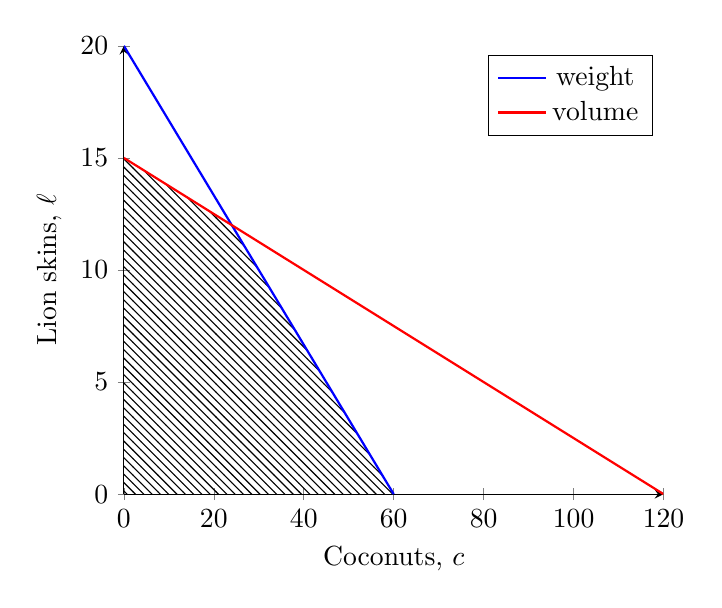
\begin{tikzpicture}
			\begin{axis}
				[
				    axis lines = left,
				    xlabel = {Coconuts, $c$},
				    ylabel = {Lion skins, $\ell$},
				]

				\addplot [
					thick,
				    domain = 0:60, 
				    samples = 100, 
				    color = blue,
				    name path = A,
				]
				{-1/3*x + 20};
				\addlegendentry{weight}

				\addplot [
					thick,
				    domain = 0:120, 
				    samples = 100, 
				    color = red,
				    name path = B,
				]
				{-1/8*x + 15};
				\addlegendentry{volume}

				\path[name path=xaxis] (\pgfkeysvalueof{/pgfplots/xmin}, 0) -- (\pgfkeysvalueof{/pgfplots/xmax},0);
				\addplot[pattern=north west lines] fill between[of=B and xaxis, soft clip={domain=0:24}];
				\addplot[pattern=north west lines] fill between[of=A and xaxis, soft clip={domain=24:60}];
			\end{axis}
			\end{tikzpicture}
			\end{center}
			We can see that the slope our of objective function is $-\frac{1}{5}$ which is bounded between $-\frac{1}{3}$ and $-\frac{1}{8}$, the slopes of our weight and volume
			constraints, respectively. Therefore, our optimal value lies at their intersection, $(24, 12)$, providing 5040 rupees.
		\end{proof}


	% problem 2
	\item[\textbf{2.}]
		\begin{enumerate}
			\item[\textbf{a.}] Formulate the \textit{Sheridan Motors} Case as a linear program whose objective is to maximize the contribution, where contribution is defined as revenue
				minus the sum of direct materials, direct labor, and variable overhead costs.
			\item[\textbf{b.}] Determine the most profitable mix of products.
			\item[\textbf{c.}] Suppose that Sheridan can obtain an additional 1000 hours per month of engine assembly capacity by renting a neighboring facility. What is the most
				Sheridan should pay for this added capacity?
		\end{enumerate}

		\begin{proof}[Solution] $ $
			\begin{enumerate}
				\item[\textbf{a.}] We are provided that following information:
					\begin{itemize}
						\item No more than 7000 machine hours for metal stamping per month.
						\item No more than 4080 machine hours for engine assembly per month.
						\item No more than 4500 machine hours for Model 101 assembly per month.
						\item No more than 4480 machine hours for Model 102 assembly per month.
						\item A Model 101 requires
						\begin{itemize}
							\item 2.8 hours of metal stamping,
							\item 1.2 hours of engine assembly,
							\item 2 hours of its own assembly,
							\item \$2134 in total to manufacture,
							\item is worth \$2100.
						\end{itemize}
						\item A Model 102 requires
						\begin{itemize}
							\item 2 hours of metal stamping,
							\item 2.4 hours of engine assembly,
							\item 3.2 hours of its own assembly,
							\item \$18 in total to manufacture,
							\item is worth \$2000.
						\end{itemize}
						\item Optimize contribution which is defined as revenue minus the sum of direct materials, direct labor, and variable overhead costs.
					\end{itemize}
					Let $x, y \in \mathbb{R}$ denote the number of Model 101's and Model 102's manufactured, respectively. Then it follows that contribution is
					$$2100x - (1200 + 200 + 400)x + 2000y - (1000 + 225 + 425)y = 300x + 350y$$
					and we obtain the following linear program.
					\begin{align*}
						\max \{ 300x &+ 350y \}  &\mathrm{objective} \\
						2.8x + 2y &\leq 7000 &\mathrm{metal\; stamping} \\
						1.2x + 2.4y &\leq 4080 &\mathrm{engine\; assembly} \\
						2x &\leq 4500 &\mathrm{101\; assembly} \\
						3.2y &\leq 4480 &\mathrm{102\; assembly} \\
						x, y &\geq 0 &\mathrm{nonnegativity}.
					\end{align*}

				\item[\textbf{b.}] Provided the linear program from \textbf{2a}, we obtain the following plot.
					\begin{center}
					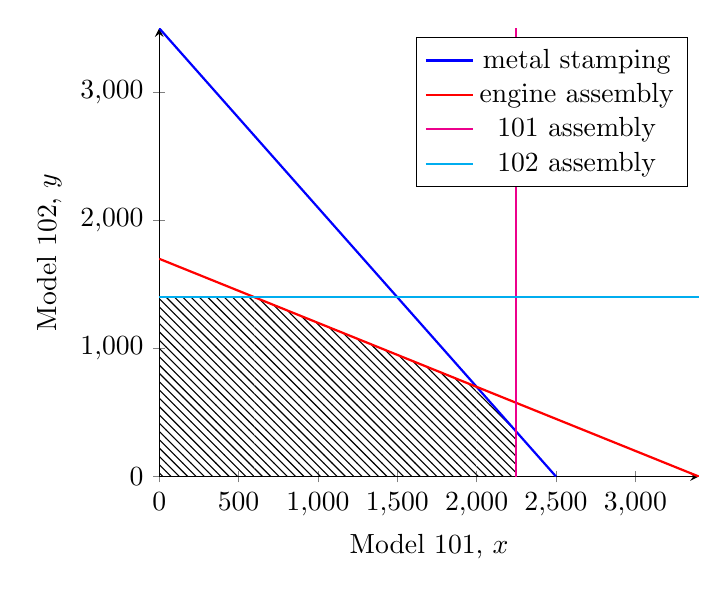
\begin{tikzpicture}
					\begin{axis}
						[
						    axis lines = left,
						    xlabel = {Model 101, $x$},
						    ylabel = {Model 102, $y$},
						]

						\addplot [
							thick,
						    domain = 0:2500,
						    samples = 100,
						    color = blue,
						    name path = A,
						]
						{-1.4*x + 3500};
						\addlegendentry{metal stamping}

						\addplot [
							thick,
						    domain = 0:3400,
						    samples = 100, 
						    color = red,
						    name path = B,
						]
						{-0.5*x + 1700};
						\addlegendentry{engine assembly}

						\addplot[thick, samples=100, domain=0:6, magenta, name path = C] coordinates {(2250,0)(2250,3500)};
						\addlegendentry{101 assembly}

						\addplot [
							thick,
						    domain = 0:3400,
						    samples = 100, 
						    color = cyan,
						    name path = D,
						]
						{1400};
						\addlegendentry{102 assembly}

				  		\path[name path=xaxis] (\pgfkeysvalueof{/pgfplots/xmin}, 0) -- (\pgfkeysvalueof{/pgfplots/xmax},0);
				  		\addplot[pattern=north west lines] fill between[of=D and xaxis, soft clip={domain=0:600}];
      					\addplot[pattern=north west lines] fill between[of=B and xaxis, soft clip={domain=600:2000}];
      					\addplot[pattern=north west lines] fill between[of=A and xaxis, soft clip={domain=2000:2250}];
					\end{axis}
					\end{tikzpicture}
					\end{center}
					We can see that the slope our of objective function is $-\frac{6}{7}$. Therefore, our optimal value lies at the vertex $(2000, 700)$ of our region
					since the corresponding slopes bound the slope of our objective function which provides \$845,000 in contribution.

				\item[\textbf{c.}] After increasing the bound of engine assembly by 1000, we obtain the following plot
					\begin{center}
					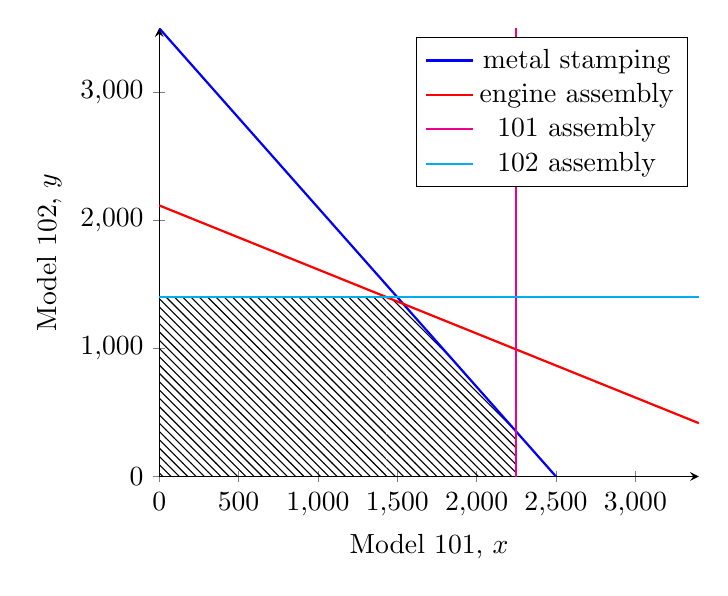
\begin{tikzpicture}
					\begin{axis}
						[
						    axis lines = left,
						    xlabel = {Model 101, $x$},
						    ylabel = {Model 102, $y$},
						]

						\addplot [
							thick,
						    domain = 0:2500,
						    samples = 100,
						    color = blue,
						    name path = A,
						]
						{-1.4*x + 3500};
						\addlegendentry{metal stamping}

						\addplot [
							thick,
						    domain = 0:3400,
						    samples = 100, 
						    color = red,
						    name path = B,
						]
						{-0.5*x + 5080/2.4};
						\addlegendentry{engine assembly}

						\addplot[thick, samples=100, domain=0:6, magenta, name path = C] coordinates {(2250,0)(2250,3500)};
						\addlegendentry{101 assembly}

						\addplot [
							thick,
						    domain = 0:3400,
						    samples = 100, 
						    color = cyan,
						    name path = D,
						]
						{1400};
						\addlegendentry{102 assembly}

				  		\path[name path=xaxis] (\pgfkeysvalueof{/pgfplots/xmin}, 0) -- (\pgfkeysvalueof{/pgfplots/xmax},0);
				  		\addplot[pattern=north west lines] fill between[of=D and xaxis, soft clip={domain=0:1433.333}];
      					\addplot[pattern=north west lines] fill between[of=B and xaxis, soft clip={domain=1433.333:1537.037}];
      					\addplot[pattern=north west lines] fill between[of=A and xaxis, soft clip={domain=1537.037:2250}];
					\end{axis}
					\end{tikzpicture}
					\end{center}
					and by the same argument, the corresponding vertex between the engine assembly and metal stamping, $(1537.037, 1348.148)$, is our optimal value providing
					\$932,962.90. Therefore, Sheridan should pay no more than \$932,962.90 - \$845,000 = \$87,962.90.
			\end{enumerate}
		\end{proof}


	% problem 3
	\item[\textbf{3.}] Consider again the \textit{Perdue Chicken} problem. Remember in that problem it was required that the quotas at each destination be met. Suppose instead that this
		requirement is loosened and it is permitted to be \textit{short} at a destination. However, a \textit{penalty cost} is incurred as follows: \$50 per ton short at New York or
		Los Angeles, \$25 per ton short at Kansas City, and \$40 per ton short at Miami. Reformulate the linear program.

		\begin{proof}[Solution]
			We are provided with the following information:
			\begin{itemize}
				\item There are 2000 tons of chickens to be distributed to New York (1), Los Angeles (2), Kansas City (3), and Miami (4).
				\begin{itemize}
					\item 500 tons in San Fransisco (1),
					\item 500 tons in Houston (2),
					\item 1000 tons in Detroit (3).
				\end{itemize}
				\item New York requires at most 300 tons with penalty of \$50 per missing ton.
				\item Los Angeles requires at most 900 tons with penalty of \$50 per missing ton.
				\item Kansas City requires at most 600 tons with penalty of \$25 per missing ton.
				\item Miami requires at most 200 tons with penalty of \$40 per missing ton.
				\item The cost of shipment per ton is
					\begin{center}
					\begin{tabular}{c|cccc}
						From$\setminus$To & New York & Los Angeles & Kansas City & Miami \\
						\hline
						San Fransisco & \$80 & \$10 & \$65 & \$80 \\
						Houston & \$30 & \$50 & \$20 & \$20 \\
						Detroit & \$30 & \$100 & \$50 & \$50
					\end{tabular}
					\end{center}
				\item Optimize shipping cost.
			\end{itemize}
			Let $a_{ij} \in \mathbb{R}$ with $1 \leq i \leq 3$ and $1 \leq j \leq 4$ denote the number of tons of chickens shipped from source city $i$ to destination city $j$.
			Similarly, let $b_{ij} \in \mathbb{R}$ denote the values in the table above for the same cities. Observe that the net profit is
			\begin{align*}
				C &= \sum_{i = 1}^3 \sum_{j = 1}^4 a_{ij}b_{ij} + 50 \left (300 - \sum_{1 = 1}^3 a_{i1} \right) + 50 \left (900 - \sum_{1 = 1}^3 a_{i2} \right) + 25 \left (600 - \sum_{1 =
					1}^3 a_{i3} \right) + 40 \left (200 - \sum_{1 = 1}^3 a_{i4} \right) \\
				&= 30a_{11} - 40a_{12} + 40a_{13} + 40a_{14} - 20a_{21} - 5a_{23} - 20a_{24} - 20a_{31} + 50a_{32} + 25a_{33} + 10a_{34}.
			\end{align*}
			Then we obtain the following linear program.
			\begin{align*}
				\min \{ &C \}  &\mathrm{objective} \\
				a_{11} + a_{12} + a_{13} + a_{14} &\leq 500 &\mathrm{San\; Fransisco} \\
				a_{21} + a_{22} + a_{23} + a_{24} &\leq 500 &\mathrm{Houston} \\
				a_{31} + a_{32} + a_{33} + a_{34} &\leq 1000 &\mathrm{Detroit} \\
				a_{11} + a_{21} + a_{31} &\leq 300 &\mathrm{New York} \\
				a_{12} + a_{22} + a_{32} &\leq 900 &\mathrm{Los\; Angeles} \\
				a_{13} + a_{23} + a_{33} &\leq 600 &\mathrm{Kansas\; City} \\
				a_{14} + a_{24} + a_{34} &\leq 200 &\mathrm{Miami} \\
				a_{ij} &\geq 0\; \mathrm{for\; all\;} i,j &\mathrm{nonnegativity}.
			\end{align*}
		\end{proof}


	% problem 4
	\item[\textbf{4.}] Formulate the rest of the following problems.
		\begin{enumerate}
			\item[\textbf{a.}] \textit{Incinerators and Pollution Control}.
			\item[\textbf{b.}] \textit{A Blending Problem}.
			\item[\textbf{a.}] \textit{Staffing a Training Program}.
		\end{enumerate}

		\begin{proof}[Solution] $ $
			\begin{enumerate}
				\item[\textbf{a.}] We are provided with the following information:
					\begin{itemize}
						\item No more than 400,000 units of sulfur dioxide can be emitted.
						\item No more than 50,000 units of particulate can be emitted.
						\item Incinerators $A, B, C$ have the following capacity and emit the following pollution.
							\begin{center}
							\begin{tabular}{c|ccc}
								 & Capacity in tons & Units of sulfur dioxide & Units of particulate \\
								Incinerator & per ton burned & per ton burned & per ton burned \\
								\hline
								$A$ & 1200 & 250 & 20 \\
								$B$ & 800 & 150 & 30 \\
								$C$ & 1000 & 220 & 24
							\end{tabular}
							\end{center}
						\item Optimize the amount of trash incinerated.
					\end{itemize}
					Let $a, b, c \in \mathbb{R}$ denote the number of tons of trash incinerated by incinerators $A, B, C$, respectively. Then we obtain the following linear program.
					\begin{align*}
						\max \{ a &+ b + c \}  &\mathrm{objective} \\
						a &\leq 1200 &A \mathrm{'s\; capacity} \\
						b &\leq 800 &B \mathrm{'s\; capacity} \\
						c &\leq 1000 &C \mathrm{'s\; capacity} \\
						250a + 150b + 220c &\leq 400,000 &\mathrm{sulfur\; dioxide} \\
						20a + 30b + 24c &\leq 50,000 &\mathrm{particulate} \\
						a, b, c &\geq 0 &\mathrm{nonnegativity}.
					\end{align*}

				\item[\textbf{b.}] We are provided with the following information:
					\begin{itemize}
						\item A one ton (2000lb) blend of steel with the following content requirements is to be produced.
							\begin{center}
							\begin{tabular}{c|cc}
								Material & At least & Not exceeding \\
								\hline
								Carbon & 3\% & 3.5\% \\
								Chrome & 0.3\% & 0.45\% \\
								Manganese & 1.35\% & 1.65\% \\
								Silicon & 2.7\% & 3\%
							\end{tabular}
							\end{center}
						\item The following materials are available to purchase.
							\begin{center}
							\begin{tabular}{c|cccccc}
								Material & Cost per pound & Carbon & Chrome & Manganese & Silicon & Availability \\
								\hline
								Pig Iron 1 (1)    & 0.03\%   & 4\%   & 0\%  & 0.9\% & 2.25\% & unlimited \\
								Pig Iron 2 (2)    & 0.0645\% & 0\%   & 10\% & 4.5\% & 15\% & unlimited \\
								Ferro-Silic 1 (3) & 0.065\%  & 0\%   & 0\%  & 0\%   & 45\% & unlimited \\
								Ferro-Silic 2 (4) & 0.061\%  & 0\%   & 0\%  & 0\%   & 42\% & unlimited \\
								Alloy 1 (5)       & 0.1\%    & 0\%   & 0\%  & 60\%  & 18\% & unlimited \\
								Alloy 2 (6)       & 0.13\%   & 0\%   & 20\% & 9\%   & 30\% & unlimited \\
								Alloy 3 (7)       & 0.119\%  & 0\%   & 8\%  & 33\%  & 25\% & unlimited \\
								Carbide (8)       & 0.08\%   & 15\%  & 0\%  & 0\%   & 30\% & 20 lb \\
								Steel 1 (9)       & 0.021\%  & 0.4\% & 0\%  & 0.9\% & 0\% & 200 lb \\
								Steel 2 (10)      & 0.02\%   & 0.1\% & 0\%  & 0.3\% & 0\% & 200 lb \\
								Steel 3 (11)      & 0.0195\% & 0.1\% & 0\%  & 0.3\% & 0\% & 200 lb
							\end{tabular}
							\end{center}
						\item Optimize the cost.
					\end{itemize}
					Let $a_i \in \mathbb{R}$ denote the number of pounds purchased of the $i^{\mathrm{th}}$ material. Then we obtain the following linear program.
					\begin{align*}
						\max \{ 0.03a_1 + 0.0645a_2 + 0.065a_3 + 0.061a_4 + 0.1a_5 &+ 0.13a_6 + \\
							+ 0.119a_7 + 0.08a_8 + 0.021a_9 + 0.02a_{10} &+ 0.0195a_{11} \} &\mathrm{objective} \\
						a_1 + a_2 + a_3 + a_4 + a_5 + a_6 + a_7 + a_8 + a_9 + a_{10} + a_{11} &= 2000 &\mathrm{total\; material} \\
						0.04a_1 + 0.15a_8 + 0.004a_9 + 0.001a_{10} + 0.001a_{11} &\geq 0.03 \cdot 2000 = 60 &\mathrm{carbon\; lower\; bound} \\
						0.04a_1 + 0.15a_8 + 0.004a_9 + 0.001a_{10} + 0.001a_{11} &\leq 0.035 \cdot 2000 = 70 &\mathrm{carbon\; upper\; bound} \\
						0.1a_2 + 0.2a_6 + 0.08a_7 &\leq 0.003 \cdot 2000 = 6 &\mathrm{chrome\; lower\; bound} \\
						0.1a_2 + 0.2a_6 + 0.08a_7 &\leq 0.0045 \cdot 2000 = 9 &\mathrm{chrome\; upper\; bound} \\
						0.009a_1 + 0.045a_2 + 0.6a_5 + 0.09a_6 + 0.33a_7 &+ 0.09a_9 + \\
							+ 0.03a_{10} + 0.03a_{11} &\geq 0.0135 \cdot 2000 = 27 &\mathrm{manganese\; lower\; bound} \\
						0.009a_1 + 0.045a_2 + 0.6a_5 + 0.09a_6 + 0.33a_7 &+ 0.09a_9 + \\
							+ 0.03a_{10} + 0.03a_{11} &\leq 0.0165 \cdot 2000 = 33 &\mathrm{manganese\; upper\; bound} \\
						0.0225a_1 + 0.15a_2 + 0.45a_3 + 0.42a_4 + 0.18a_5 &+ 0.3a_6 +\\
							+ 0.25a_7 + 0.3a_8 &\geq 0.027 \cdot 2000 = 54 &\mathrm{silicon\; lower\; bound} \\
						0.0225a_1 + 0.15a_2 + 0.45a_3 + 0.42a_4 + 0.18a_5 &+ 0.3a_6 + \\
							+ 0.25a_7 + 0.3a_8 &\geq 0.03 \cdot 2000 = 60 &\mathrm{silicon\; upper\; bound} \\
						a_8 &\leq 20 &\mathrm{carbide\; availability} \\
						a_9 &\leq 200 &\mathrm{steel\; 1\; availability} \\
						a_{10} &\leq 200 &\mathrm{steel\; 2\; availability} \\
						a_{11} &\leq 200 &\mathrm{steel\; 3\; availability} \\
						a_i &\geq 0\; \mathrm{for\; all\;} i &\mathrm{nonnegativity}.
					\end{align*}

				\item[\textbf{c.}] We are provided with the following information:
					\begin{itemize}
						\item Agents are available 120 hours a month and they can either train students for 20 hours or serve the public.
						\item The monthly demand of public service from the agents is
							\begin{center}
							\begin{tabular}{c|c}
								Month & Demand in hours \\
								\hline
								January & 8000 \\
								February & 9000 \\
								March & 7000 \\
								April & 10,000 \\
								May & 9000 \\
								June & 11,000
							\end{tabular}
							\end{center}
						\item From the beginning of the year, 60 trained agents are initially availability.
						\item Payroll costs per month are
							\begin{center}
							\begin{tabular}{cc}
								Student: & \$350 \\
								Trained agent: & \$600
							\end{tabular}
							\end{center}
						\item Optimize the cost.
					\end{itemize}
					Let $h_i \in \mathbb{R}$ denote the number of hired and trained agents in month $1 \leq i \leq 6$. Similarly, let $a_i \in \mathbb{R}$ denote the number of trained
					agents available at the beginning at the $i^{\mathrm{th}}$ month. Then we can see that $a_1 = 60$ and $$a_{i + 1} = a_i + h_i = 60 + \sum_{j = 1}^i h_j$$ for all $1
					\leq i \leq 5$. Observe that the cost can be represented as
					\begin{align*}
						C &= 350\sum_{i = 1}^6 h_i + 600\sum_{i = 1}^6 a_i \\
						&= 350\sum_{i = 1}^6 h_i + 600\sum_{i = 1}^6 \left ( 60 + \sum_{j = 1}^{i-1} h_j \right ) \\
						&= 36,000 + 350\sum_{i = 1}^6 h_i + 600\sum_{i = 1}^5 \sum_{j = 1}^i h_j \\
						C &= 36,000 + 3350h_1 + 2750h_2 + 2150h_3 + 1550h_4 + 950h_5 + 260h_6. \\
					\end{align*}
					Additionally, we need $$120a_i - 20h_i = 120\left ( 60 + \sum_{j = 1}^{i-1} h_jc\right ) - 20h_i$$ to meet the $i^{\mathrm{th}}$ monthly demand. Then we obtain the
					following linear program.
					\begin{align*}
						\min \{ &C \} &\mathrm{objective} \\
						7200 - 20h_1 &\geq 8000 &\mathrm{January\; demand} \\
						7200 + 120h_1 - 20h_2 &\geq 9000 &\mathrm{February\; demand} \\
						7200 + 120h_1 + 120h_2 - 20h_3 &\geq 7000 &\mathrm{March\; demand} \\
						7200 + 120h_1 + 120h_2 + 120h_3 - 20h_4 &\geq 10,000 &\mathrm{April\; demand} \\
						7200 + 120h_1 + 120h_2 + 120h_3 + 120h_4 - 20h_5 &\geq 9000 &\mathrm{May\; demand} \\
						7200 + 120h_1 + 120h_2 + 120h_3 + 120h_4 + 120h_5 - 20h_6 &\geq 11,000 &\mathrm{June\; demand} \\
						h_i &\geq 0\; \mathrm{for\; all\;} i &\mathrm{nonnegativity}.
					\end{align*}
			\end{enumerate}
		\end{proof}

\end{enumerate}

\end{document}
